\documentclass[class=article]{standalone}

%\documentclass[12pt, a4paper]{article}
%
%\usepackage{../preambolo}

\begin{document}
%	\justifying	
	\section{Raccolta Dati}
	In questo capitolo verranno descritte le sessioni di raccolta dati e verrà fornita una \\panoramica dei dati stessi.
	
	\subsection{Gli Esperimenti}
	La raccolta dati è avvenuta in diverse sessioni, ognuna delle quali si è focalizzata su una differente situazione di guida. In particolare sono stati prese in considerazione le fasi di:
	\begin{itemize}
		\item accelerazione: in questa fase i dati sono stati raccolti sia durante una situazione di pedalata normale che forte in un percorso rettilineo
%		\item lieve accelerazione: in questa fase i dati sono stati raccolti emulando una situazione di pedalata normale
%		\item forte accelerazione: in questa fase i dati sono stati raccolti emulando una situazione di pedalata vigorosa
		\item frenata: in questa fase i dati sono stati raccolti sia in situazioni di progressiva che di repentina perdita di velocità
		\item curva: in questa fase sono stati raccolti dati inerenti a curve principalmente di 90° e 180° percorse più o meno velocemente
	\end{itemize}
	
	Dato che il sensore non era integrato sulla bicicletta, ma andava fissato di volta in volta sulla stessa, all'inizio di ogni sessione è stato necessario determinare la matrice di rotazione da applicare ai dati per far coincidere il sistema di riferimento del sensore con quello della bicicletta. Per far ciò, una volta fissato il sensore, sono stati raccolti dati per un periodo di tempo di \(30s\) con la bicicletta mantenuta ferma dapprima in posizione verticale (in modo che la direzione dell'asse longitudinale fosse parallelo al terreno) e, successivamente, inclinata. Dei dati così raccolti sono stati tenuti i \(10s\) centrali, in modo da eliminare gli istanti successivi all'accensione e precedenti allo spegnimento del sensore, che sono i più sporchi. I primi dati ottenuti, quelli con la bicicletta in verticale, sono stati quindi utilizzati per calcolare la rotazione attorno all'asse \(x\). Questo è stato fatto calcolando il modulo del valor medio della componente gravitazionale che giace sul piano \(yz\) e calcolando poi la rotazione necessaria per annullare la componente \(x\) di tale vettore.
	
	\[\theta_{x}=acos\left(\frac{g_{z}}{|g_{yz}|}\right)\]
	con \(\theta_{x}\) la rotazione attorno all'asse \(x\), \(g_{z}\) la componente gravitazionale lungo l'asse \(z\) e \(|g_{yz}|\) il modulo del vettore composto dalle componenti \(y\) e \(z\) del vettore gravità. È stata quindi ottenuta la prima matrice di rotazione \(M_{x}\)
	
	\[M_{x}= \begin{bmatrix}
		1 & 0 & 0 \\
		0 & cos(\theta_{x}) & -sin(\theta_{x}) \\
		0 & sin(\theta_{x}) & cos(\theta_{x})
	\end{bmatrix}\]
	Allo stesso modo è stata poi ottenuta la rotazione attorno all'asse \(y\) e la rispettiva matrice di rotazione \(M_{y}\). Infine, grazie al secondo set di dati, quello con la bicicletta inclinata, è stato possibile ottenere la rotazione attorno all'asse \(z\) e la matrice \(M_{z}\).
	
	\[M_{y}=\begin{bmatrix}
		cos(\theta_{y}) & 0 & sin(\theta_{y}) \\
		0 & 1 & 0 \\
		-sin(\theta_{y}) & 0 & cos(\theta_{y})
	\end{bmatrix}\]
	
	\[M_{z}=\begin{bmatrix}
		cos(\theta_{z}) & -sin(\theta_{z}) & 0 \\
		sin(\theta_{z}) & cos(\theta_{z}) & 0 \\
		0 & 0 & 1
	\end{bmatrix}\]
	
	La matrice di rotazione complessiva è stata poi ottenuta moltiplicando le singole matrici di rotazione 
	
	\[M=M_{x}\cdot M_{y}\cdot M_{z}\]
	ed è stata applicata ai dati raccolti per portarli nel sistema di riferimento della bicicletta.
	
	\begin{center}
		\begin{figure}[h]
			\centering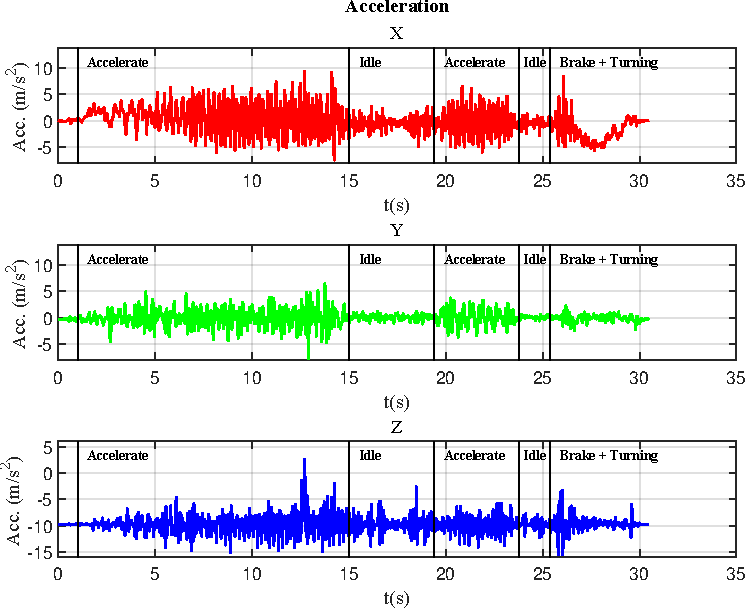
\includegraphics[width=.9\textwidth]{img/Acc LungaF.pdf}
			\caption[]{Grafico dei dati di accelerazione raccolti durante un percorso rettilineo. Dalle immagini si può notare come nelle fasi di accelerazione (\(Accelerate\))  lungo gli assi \(X\) e \(Y\) siano più ampie rispetto alle fasi di \(idle\).}
			\label{fig:AccLunga}
		\end{figure}
	\end{center}
	
	\subsection{Dati Raccolti}
	Durante i vari esperimenti il sensore ha raccolto i dati di accelerazione, velocità angolare e campo magnetico con una frequenza di campionamento di \(25Hz\) (un campione ogni \(0.04s\)). In questa sezione verrà trattato di come si comportano queste grandezze durante i vari esperimenti fatti.
	
	
	\begin{center}
		\begin{figure}[h]
			\centering\includegraphics[width=.9\textwidth]{img/Vang LungaF.pdf}
			\caption[]{Grafici dei dati delle velocità angolari raccolti durante un percorso rettilineo. Dalle immagini si può notare come nelle fasi di \(Accelerate\) le oscillazioni degli angoli \(roll\) e \(yaw\) siano più ampie rispetto alle fasi di \(idle\).}
			\label{fig:VAngLunga}
		\end{figure}
	\end{center}
	
	\subsubsection{Accelerazione}
	Le fasi accelerazione si sono svolte su un percorso rettilineo. Durante queste fasi, delle tre grandezze considerate, solo l'accelerazione e la velocità angolare hanno prodotto variazioni apprezzabili.
	
	In particolare, l'accelerazione lungo l'asse \(x\) risulta oscillante, con oscillazioni tanto più elevate quanto più il ciclista pedala intensamente. Queste oscillazioni sono dovute, come discusso nel capitolo riguardante la fisica della bicicletta, dall'azione del piede sul pedale e dal fatto che non è possibile riuscire a imprimere costantemente la massima forza ma questa dipende dall'orientamento della pedivella. La forza applicata nel pedalare si traduce anche in un'oscillazione della bicicletta, visibile sia sull'accelerazione lungo l'asse \(y\) che in una rotazione attorno all'asse \(x\) (\(roll\)).
	
	Nei dati provenienti dal giroscopio è inoltre possibile osservare una rotazione attorno all'asse z (\(yaw\)) tanto maggiore quanto il ciclista si "impegna" nel pedalare. Questo è dovuto all'azione del ciclista sul manubrio per mantenere in equilibrio la bicicletta.
	
	In tutti i casi precedenti l'oscillazione cessa quando il ciclista smette di pedalare e procede per inerzia.
	
	\begin{center}
		\begin{figure}[h]
			\centering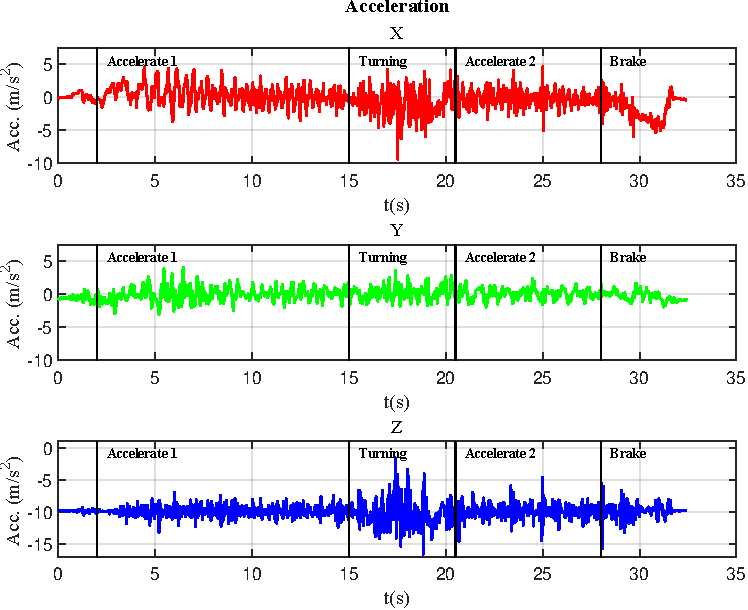
\includegraphics[width=.9\textwidth]{img/Acc CurvaUF.pdf}
			\caption[]{Grafico dei dati di accelerazione raccolti durante un percorso con curva a U. Dalle immagini si può notare come, nella fase di curva (\(Turning\)), vi sia un abbassamento dell'andamento medio dell'accelerazione in \(X\).}
			\label{fig:AccCurvaU}
		\end{figure}
	\end{center}
	
	\subsubsection{Frenata}
	Durante le fasi di frenata l'accelerazione l'ungo l'asse \(x\) decresce rapidamente e diventa negativa a causa dell'azione del freno, in maniera più o meno marcata, a seconda dell'intensità della frenata.
	
	In caso di frenate particolarmente intense, è inoltre possibile notare l'effetto della frenata anche come rotazione attorno all'asse \(y\). Questo è dovuto all'inerzia del ciclista che, facendogli spostare il peso in avanti, causa un'inclinazione della bicicletta.
	
	\begin{center}
		\begin{figure}[h]
			\centering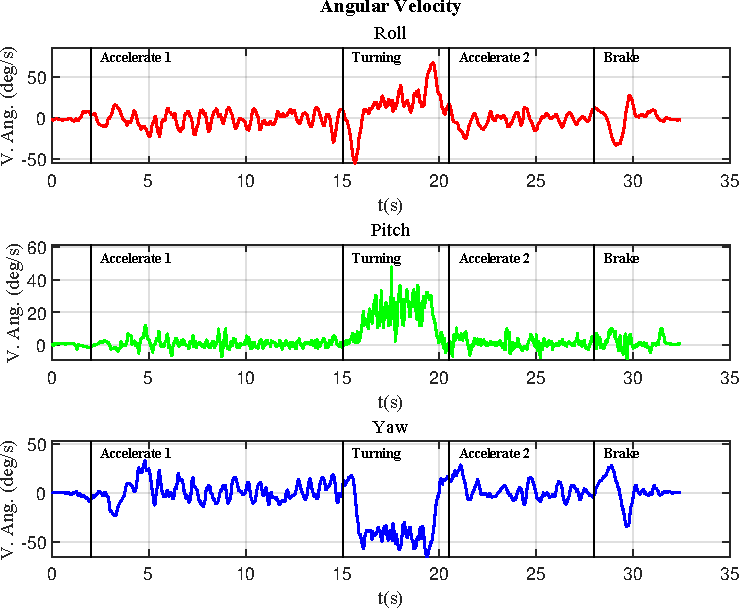
\includegraphics[width=.9\textwidth]{img/VAng CurvaUF.pdf}
			\caption[]{Grafico dei dati di velocità angolare raccolti durante un percorso con curva a U. Dalle immagini si può notare un picco all'inizio e alla fine della curva (\(Turning\)) attorno all'angolo di rollio (\(Roll\)). Negli altri angoli, invece, si può notare in incremento/decremento del loro valore durante la curva.}
			\label{fig:VAngCurvaU}
		\end{figure}
	\end{center}
	
	
	\subsubsection{Curva}	
	Durante le curve le misure di accelerazione diventano meno rilevanti, si assiste principalmente a una riduzione della componente in \(x\).
	
	Le velocità angolari, invece, mostrano variazioni significative. All'inizio e alla fine delle curve si osservano due picchi di verso opposto nell'angolo di rollio, più o meno pronunciati a seconda dell'inclinazione della bicicletta durante la curva.
	Quest'inclinazione causa anche a un aumento dell'angolo di beccheggio (\(pitch\)) dovuto alla rotazione della bicicletta attorno all'asse \(y\) durante la curva.
	Inoltre, il valore dell'angolo di imbardata (\(yaw\)) aumenta o decresce a seconda del verso della curva (se si ruota in senso orario o antiorario).
		
	Anche il campo magnetico, che finora non era stato particolarmente rilevante, riesce a fornirci importanti informazioni. Infatti, il magnetometro, agendo come una bussola, ci dice molto riguardo all'orientamento della bicicletta. In particolare l'asse \(x\), durante la curva, subisce un rapido aumento o diminuzione a seconda di dove si colloca il nord magnetico terrestre rispetto alla bicicletta.
	
	\begin{center}
		\begin{figure}[h]
			\centering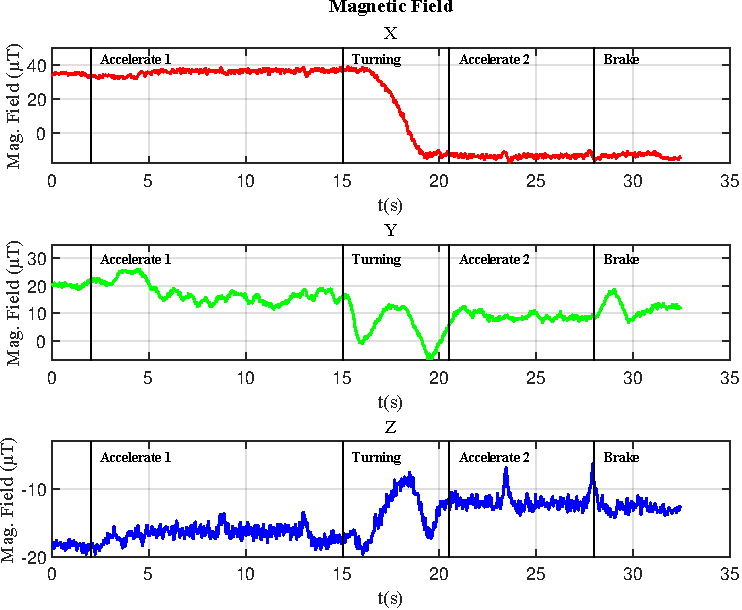
\includegraphics[width=.9\textwidth]{img/Mag CurvaUF.pdf}
			\caption[]{Grafico dei dati del campo magnetico raccolti durante un percorso con curva a U. Dalle immagini si può notare un deciso abbassamento del campo magnetico in \(X\) dovuto al cambiamento di direzione.}
			\label{fig:MagCurvaU}
		\end{figure}
	\end{center}
%	\subsection{To Do?}
%	Magari aggiungere:
%	\begin{itemize}
%		\item qualcosa sulla bicicletta
%		\item qualcosa sulla strada dove sono stati raccolti i dati
%		\item accenni alla velocità
%		\item (integrale della velocità angolare?)
%		\item Trasformata e spettro
%	\end{itemize}
		
\end{document}